\chapter{Iterative Appliation Design (contributions)}
\label{cha:contributions}

This chapter describes the contributions of all papers that are included in the thesis and them to the descriptions about application design as described in the previous chapter. The following sections first describe the separation of papers into topic areas and then elaborate on each of the topics.

\section{Overview}
\label{contributions:overview}
Due to the varied nature of application papers, this papers are separated into three topic areas:

\textbf{Biological and Medical Visualization. } \paperef{paperA} and \paperef{paperB} deal with algorithmic and application design challenges regarding biological simulation and medical intervention support respectively. \paperef{paperA} describes an algorithm that was developed to effieciently render non-linear finite element models; \paperef{paperB} describes an application system used in deep brain stimulation interventions.~(\SC{contributions:medbio})

\textbf{Urban Search \& Rescue. } \paperef{paperC}, \paperef{paperD}, and \paperef{paperE} describe the collaborative work on designing a visualization system to support urban search \& rescue operators and rescuers. The system utilizes \nD{3} point cloud data as the basis for a pathfinding algorithm, whose results are presented to the expert user for a human-in-the-loop decision support.~(\SC{contributions:usar})

\textbf{Astrophysical Phenomena. } The papers in this topic deal with visualization system that were performed to deal with astronomical and astrophysical phenomena. \paperef{paperF} and \paperef{paperH} describe visualization systems that are applied to space weather and ion simulations respectively, where as \paperef{paperG} describes the required algorithm necessary to achieve these systems.~(\SC{contributions:physics})

Each of the topics provides a short introduction into the domain and, then, elaborate on the work that has been done in the respective papers.

% For each contribution explain:
%   Problem domain
%   System that solves the problem
%   Collaboration with the experts
%   Evaluations
%   Generalizability (future work?)

\section{Biological and Medical Systems}
\label{contributions:medbio}
\begin{itemize}
\item Describe background and previous work in biological visualization + systems
\item Describe background and previous work in medical visualization + systems
\item Medical visualization as one of the first expert domains
\item Support for the operating theater
\item General problems with medical visualization
\begin{itemize}
    \item Hard to convince people to use it:
    \item Certification / limited time of the physicians
\end{itemize}
\item More information about medical visualization \cite{preim2007visualization}
\end{itemize}

\subsection{Finite Element Visualization}
\label{contributions:medbio:fem}
In this project we developed an algorithm for real-time volume rendering of multi-variate non-linear finite element model~(FEM) simulation of a human heart. These simulations calculate the stress tensor at each location during a cardiac cycle. By comparing the results of a patient's response with the architypical heart, it becomes possible to detect structural defects before they manifest~\cite{young1992three, young1995tracking}. Traditionally, these models are visualized using iso-surfaces or glyphs~\cite{wunsche2003visualization}, but not using volume rendering. As was stated in \SC{introduction:volumerendering}, the value for each sampling point during the volume ray marching has to be fetched for a correct front-to-back compositing. This step becomes a bottleneck in the case of non-linear FEM datasets, as the data access becomes non-trivial, thus reducing rendering speeds to non-interactivity. \paperef{paperA} describes an algorithm that utilizes a precomputation step to cache a reduced set of possible rays that are then used at rendering time to efficiently access the data, resulting in a 15$\times$ performance gain, relative to straight-forward GPU implementations, which in turn, is an improvement of 2 to 4 orders of magnitude compared to a straight-forward CPU implementation~\cite{Liu12Fem}. 

\subsubsection{Background}
\label{contributions:medbio:fem:background}
FEM methods are used extensively in a large number of fields, for example engineering, construction, or biology, as an approach to solve problems numerically. For these methods, the problem domain is separated into a finite number of cells over which the numerical simulation can be performed. For more information, we refer the reader to the book by Bathe and Wilson~\cite{bathe1976numerical}. For our purposes it suffices to know that each element is associated with at least two coordinate systems. The location and deformation of each element is specified in (usually Cartesian) \emph{world coordinates}, denoted by $\vec{x}$ in $\rthree$, whereas the values it contains are stored in a material coordinate system $\xi$ which, in most cases, is of a simple geometry such as cubes, triangles, or tetrahedra. The variates of study are defined in the material coordinate space and are interpolated using trilinear interpolation. The transformation between world coordinates and material coordinates can be arbitrarily complex and undoing these transformations is at the heart of the mission performance to be able to render these models interactively using volumetric rendering techniques.

\subsubsection{Algorithm}
\label{contributions:medbio:fem:algorithm}

\subsubsection{Generalization}
\label{contributions:medbio:fem:generalization}


\begin{itemize}
\item Rendering multi-variate non-linear finite element models
\item Transformation from linear rays in world-space to curve rays in material space
\item Simulation values are described in material space
\item Transformation from world to material space is computationally expensive (multi-dimensional Newton method requires multiple iterations involving the Jacobian)
\item Solve by using precomputation step to compute proxy rays for each element
\item Precomputation is allowable as the elements are usually not degenerate and smooth
\item During rendering time, proxy rays are used to look up values in the finite elements and perform the ray marching
\item Proxy ray computation
\item Voreen: \cite{meyer2009voreen}
\begin{itemize}
    \item Create a uniform grid on the surfaces of each element
    \item Compute rays from each grid cell to each other grid cell
    \item Collect all proxy rays and store a limited number of control points used for Catmull-Rom spline interpolation 
    \item Move them into a common coordinate system (one point into origo, linear scaling, rotating all splines such that P0, Pp, Pn lie in the yz plane [P0 and Pn already on z axis from normalization], Pp is the first non-collinear point). Store $\theta$ from the rotation
    \item Perform clustering on the proxy rays \cite{abraham03clustering} with K-means \cite{hartigan75kmeans}
    \item Metric for clustering is the area covered between two splines
    \item Allow for potential different grid resolutions on entry v exit faces -> importance-based ray sampling
\end{itemize}
\item Rendering
\begin{itemize}
    \item Depth peeling \cite{mammen89DepthPeeling}
    \item Lookup ray id and $\theta$
    \item Bend and rotate closest ray into place
    \item Perform ray marching along the proxy ray (arc parametrization to take into account the different lenghts in material and world space \cite{guenter90arclength})
    \item Intersegment handling of sampling points (we do not want to start the sampling at the beginning, but have a continuous transition between elements)
    \item Inter vs intra ray interpolation
    \begin{itemize}
        \item Inter: bilinear lookup between four closest ray matches and perform interpolation between spline results
        \item Intra: Retrieving the opposite ray (entry->exit; exit->entry) and looking up at $t$ and $1-t$ and interpolate between
    \end{itemize}
\end{itemize}

\end{itemize}

\subsection{Deep Brain Stimulation Interventions}
\label{contributions:medbio:dbs}
\question{Is this too much a retelling of the paper story? If so, what additional information should be in here?}
In we work package of \paperef{paperB}, the task was to develop a medical visualization application for deep brain stimulation (DBS) intervention support in collaboration with physicians at the St.~Barbara Hospital in Hamm, Germany. This system should be designed to support the brain surgeon during the surgery in order to achieve a higher precision and thus a higher probability of a positive outcome for the patient. In contrast to other medical domains, where the doctor's available preparation time for each patient is limited and thus procludes any complex interaction techniques on visualization applications, DBS interventions already have a long planning phase scheduled prior to the operation, thus enabling the usage of specialized tools and providing the ability for visualization to play an important role in this scenario.

The application resulting from this collaboration combines an enhanced multimodal \nD{3} volumetric rendering environment with the spatial visualization of electric measurements that are recording the patient's brain activity during the procedure in combination with patient-specific ability tests. Spatially embedding the measurements with the volumetric information reduces the cognitive load of the surgeon during the surgeon, as this mental link does not have to be performed by the surgeon themself. Furthermore, the system shows the uncertainties of the different modalities in a single view, thus enabling the surgeon a comprehensive view and  more insight during the procedure.

\subsubsection{Background}
\label{contributions:medbio:dbs:background}
With the system, we target DBS interventions that are performed on patients' afflicted with Parkinson's Disease or other forms of essential tremors. During these interventions, a stimulating electrode is inserted into patients' brains that has the potential to inhibit some of the debilitating effects of these tremors~\cite{Lindberg2002}. A potential beneficial target region for the electrode locaiton is the patient's subthalamic nucleus~(STN)~\cite{Benabid2009}. However, the STN is a relatively small structure with the size of a few millimeters~\cite{Richter2004} and a location deep inside the patient's brain. Furthermore, it not detectable in MRI scans in some patients~\cite{Starr2002} and thus hard to localize. The intervention is further complicated as a small deviation in the electrode's location will excite other parts of the patient's brain that can lead to undesired memory or speech impairments.

In addition to traditional imaging modalities, the system makes use of Microelectrode Recordings~(MER)~\cite{Lenz1988} capable of recording the electrical activities in different parts of the brain. The MER system consists of a small group of electrodes that measure the brain's electric field around them. The relative amplitude and frequency of these fields correlate with the specific brain region that the electrode is in~\cite{benazzouz2002intraoperative} and can thus be used to determine whether the electrodes are in the correct locations inside the patient's brain. The results of the MER recordings are traditionally reviewed on loudspeakers that are placed in the operating room. Aside from the obvious drawbacks of a limited auditory channel, potential background noise, and limited echoic memory, a big issue is the surgeon's mental separation between the spatial location of the electrodes and their measurements. This holds true for both the absolute location of the electrode cluster inside the brain, as well as the relative positions of the electrodes inside the cluster.

Problems that were not sufficiently solved by previous methods include the fusion of the available modalities. These modalities include pre-operative CT and MRI scans, interoperative X-Ray scans, the electrode measurements during the insertion, and patient tests after the final electrode has been activated. Making efficient use of all available information is important as the principal limiting factor for the maximum operation length is the patient's ability to cooperate, as a DBS intervention is very taxing to the patient as they have to be awake during the entire procedure which can last up to 10 hours.

A DBS procedure is split into three distinct phases. In the first phase, the \emph{planning} phase, the surgeon plans the operation by locating and segmenting the most probable location of the STN using preoperative CT and MRI scans. Using other tools~\cite{Shamir2010}, an optimal access channel is then planned that evades important sensitive brain regions and selects the optimal location for the electrode to affect the STN~\cite{butson2007patient}. In the second phase, the \emph{recording} phase, the patient is in the operating room with their head in a stereotaxic frame, that restricts the movement and thus allows for a fixed-body transformation between the patient and the operating room, used for later registration. The MER sensors are inserted into the patient's brain along the preplanned access path until they have reached the planned depth. During this phase, the measurements of the electrodes are used to distinguish the different adjacent brain regions. If the electrodes correctly identify the STN region, the depth along the access path is noted and the electrodes' location is verified with bi-planar X-ray scans. After this verification, the electrodes are retracted. In the third phase, the \emph{placement} phase, a transmitting electrode is inserted into the access path to the same location that was measured during the previous phase. Once the electrode is in place, it is activated and its output is tuned. Using interoperative bi-planar X-ray scans and markers on the stereotactic frame, the location of the electrode inside the patient's brain is verified. Then, utilizing patient tests that examine the patients' ability, such as long term memory ability and measuring the tremor, the location of the electrode might be adjusted until an acceptable response is achieved or the patient is no longer capable of coorperating due to the length of the procedure.

\subsubsection{System}
\label{contributions:medbio:dbs:system}
\question{Should I use ``I'' or ``we'' in the text?}
\begin{figure}
\fbox{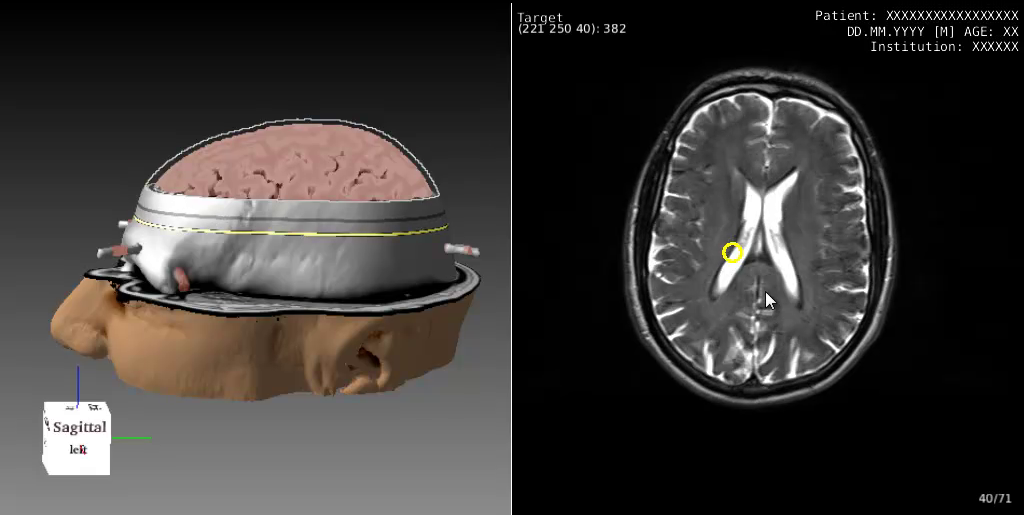
\includegraphics[width=\linewidth]{figures/contributions/dbs/planning.png}}
\caption{This view shows the part of the system that is used to import the results of a different planning tool to determine the entry point for the access path and the intented target location.}
\label{contributions:medbio:dbs:planning}
\end{figure}

In close collaboration with the surgeons, we created a system that can ingest the access path planned using other sophisticated tools (see~\fref{contributions:medbio:dbs:planning}), the various scans (T$_1$ and T$_2$ MRI, CT, and X-Ray), the MER measurements, as well as the patient tests during the operation. Combining all available modalities into one system enables the surgeon to inspect all available information for both operational phases. The system consists of multiple linked views. The \emph{Contextual view} is available in both phases, whereas the \emph{2D audio visualization} and \emph{3D audio visualization} are only available in the recording phase and the \emph{Target closeup} and \emph{Placement guide} are only available in the placement phase. The rest of this section elaborates on the design decisions for the individual views.

\question{How detailed should this be?}
\begin{figure}
\centering
\begin{subfigure}[b]{0.49\linewidth}
    \fbox{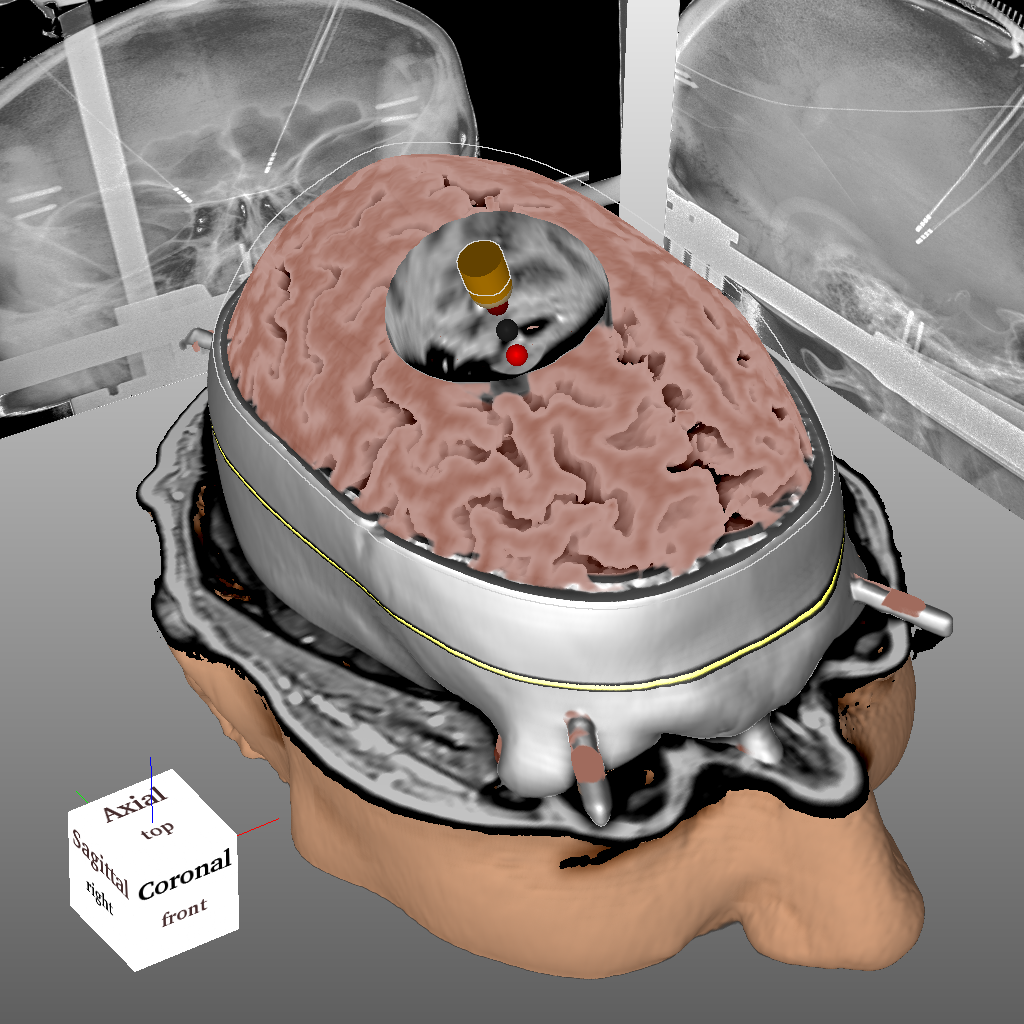
\includegraphics[width=\linewidth]{figures/contributions/dbs/recording-3d-1.png}}
\end{subfigure}
\hfill
\begin{subfigure}[b]{0.49\linewidth}
    \fbox{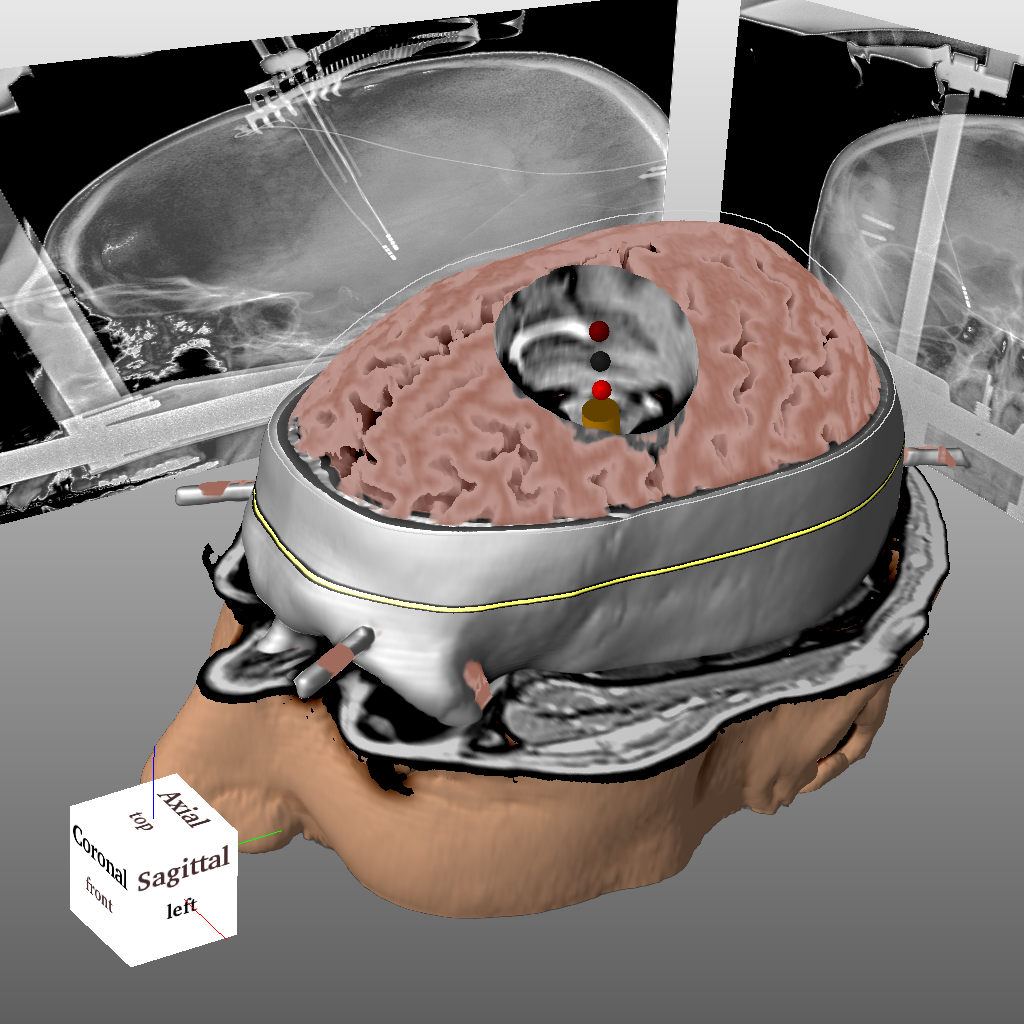
\includegraphics[width=\linewidth]{figures/contributions/dbs/recording-3d-2.png}}
\end{subfigure}
% \includegraphics[width=\linewidth]{figures/contributions/dbs/recording-3d.png}
\caption{Presenting the \emph{Contextual View} that shows the multimodal fusion of all available datasets. The preoperative CT and MRI as well as the interoperative bi-planar X-ray scans are visible together with the animated location of the electrode. The colored beads along the access path show an automatic classification of the electrode measurements.}
\label{contributions:medbio:dbs:contextual}
\end{figure}

\paragraph{Contextual View} This \nD{3} view combines the preoperational CT and MRI scans together with the bi-planar X-rays and the current electrode location (see~\fref{contributions:medbio:dbs:contextual}). For improvide depth perception, we utilize a depth darkening effect as presented by Luft~\etal~\cite{luft2006image}. The selected access path is presented in this view as a carved out tunnel along which the electrode is moved during the operation. Explicitly showing the access path serves two purposes, first, it reduces the chance of a dangerous left-right mismatch error that might otherwise occur in the operation in which the electrode is accidentally inserted into the wrong hemisphere. Second, it enables us to place colored beads inside the access path behind the electrode. The colors of these beads depend on an automatic region classification of the incoming electrode signal. This method was adopted from related works~\cite{Haese2005, Miocinovic2007}.

\paragraph{2D audio visualization} This view shows an augmented visualization similar to an oscilloscope that presents the direct measurements from the available electrodes. As only the amplitude and frequency are important during the procedure, we emphasize measurements that exceed a user-defined threshold and deemphasize the values below the threshold (see~\fref{contributions:medbio:dbs:sound:2d}). By this technique we highlight the potentially important measurements and reducing the visual noise from the low intensity signals. This view is linked with the \emph{3D audio visualization}, described below, such that when a specific electrode is selected in either view, it is highlighted in both views with a different color. This can be used by the surgeon to be able to correlate the detailed measurements with the relative location of the electrode.
\begin{figure}
\centering
    \begin{subfigure}[b]{0.49\linewidth}
        \fbox{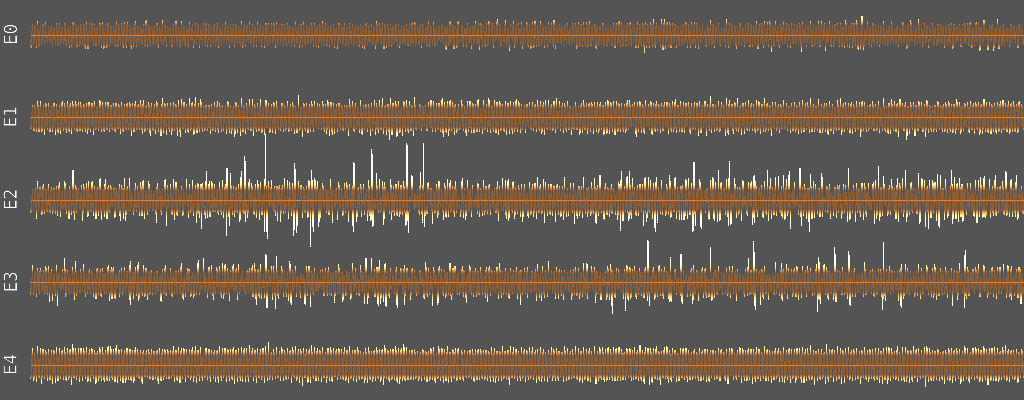
\includegraphics[width=\linewidth]{figures/contributions/dbs/audio-signal.png}}
        \caption{The \nD{2} oscilloscope rendering of the direct electrode measurements. Measurements with low amplitude are deemphasized by using darker colors.}
        \label{contributions:medbio:dbs:sound:2d}
    \end{subfigure}
    \hfill
    \begin{subfigure}[b]{0.49\linewidth}
        \fbox{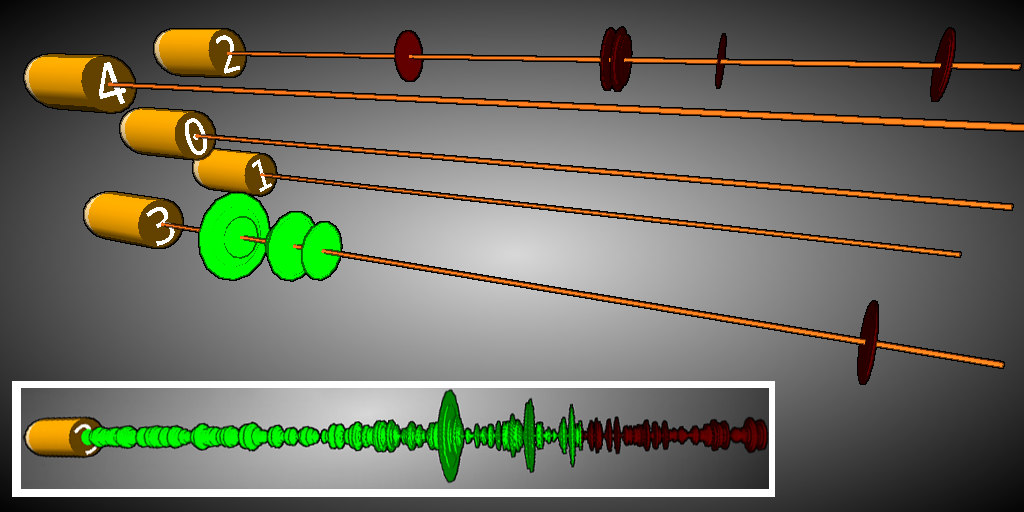
\includegraphics[width=\linewidth]{figures/contributions/dbs/recording-3dsound.png}}
        \caption{The spatial \nD{3} rendering of the electrode rendering, showing their relative spatial location and rendering the high-amplitude measurements of the signal as colored discs.}
        \label{contributions:medbio:dbs:sound:3d}
    \end{subfigure}
    \caption{This figure shows the two rendering methods for displaying the measurements recorded by the Microelectrode Recording electrodes. Both a view containing the accurate values are available (a) as well as a view showing the relative spatial relation between the electrodes.}
    \label{contributions:medbio:dbs:sound}
\end{figure}

\paragraph{3D audio visualization} In this separate view, the relative locations of the different electrodes are displayed (see~\fref{contributions:medbio:dbs:sound:3d}). The camera orientation is linked between this and the \emph{Contextual View} such that the mental registration between the two views is not broken. In this view, each electrodes' measurements that exceed a user-defined threshold are shown as discs that start at the electrode and move away from the electrode's base with increasing time. The size of the disc corresponds to the amplitude of the detected signal and thus shows the strength of the measured signal. This allows the surgeon to view the two important values (amplitude and frequency) for each of the electrodes together with their spatial orientation. The color of each disc is determined by the same classification algorithm that is used on the beads in the \emph{Contextual View}, but is simplified to show red if the electrode is outside of the STN and green if it is inside the STN. The surgeon can then, by correlating the frequency of discs and their amplitude verify that the classification was correct and that the electrodes are in the correct location.

\begin{figure}
\fbox{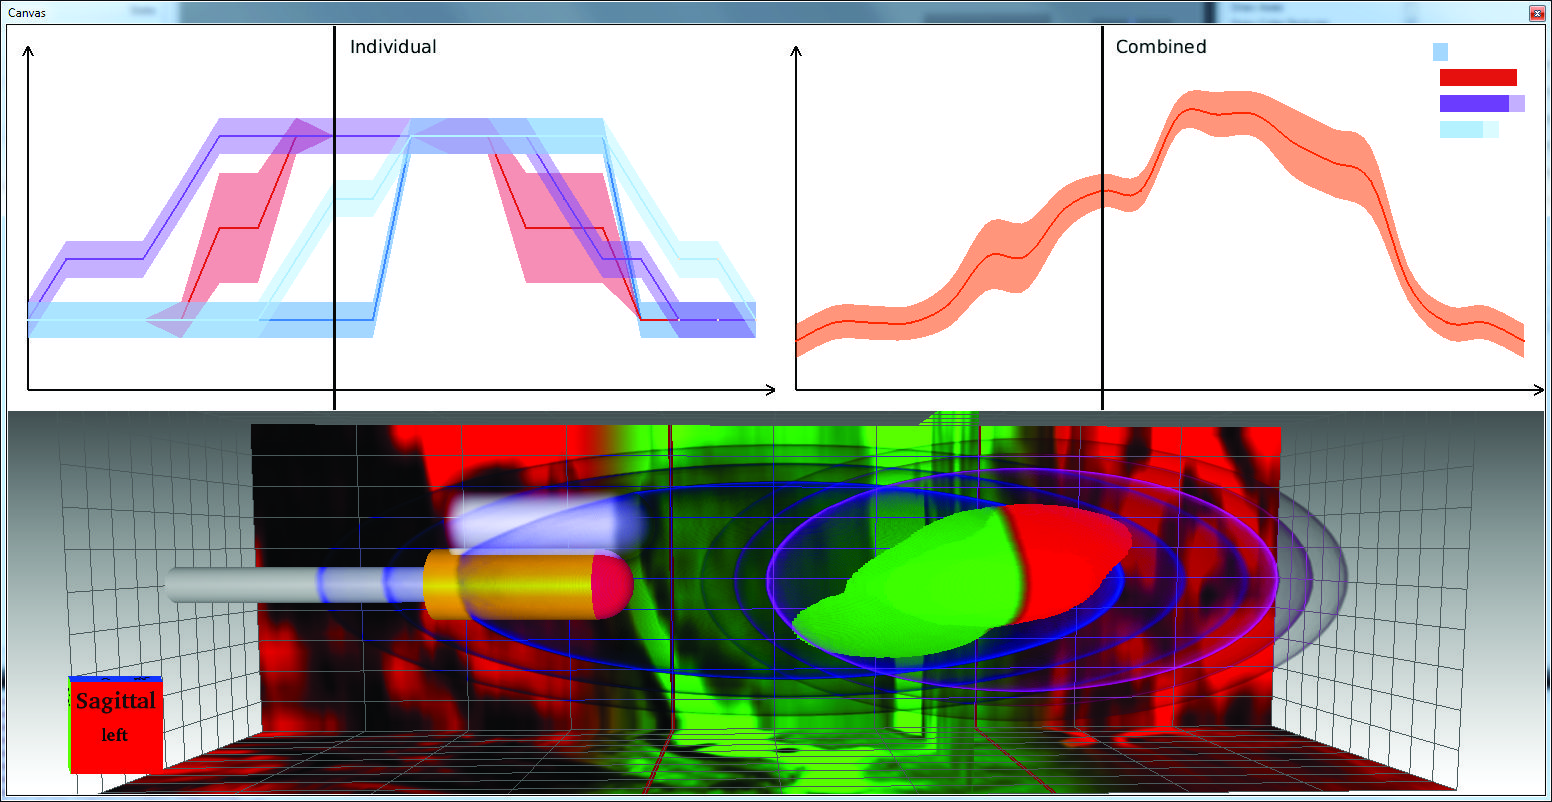
\includegraphics[width=\linewidth]{figures/contributions/dbs/screenshot-target.jpg}}
\caption{The views that show the results of the different measurements performed during the recording phase. The \emph{Target closeup} (bottom view) contains the segmented location of the STN is visible as well as the results of the different tests at their spatial location. The \emph{Placement guide} shows the likelihood measurements according to their depth along the access path}
\label{contributions:medbio:dbs:target}
\end{figure}

\paragraph{Target closeup} After the potential electrode location has been determined, the surgeon uses this closeup view, centered around the segmented location of the STN, that combines all of the information that was gathered in the recording phase (see~\fref{contributions:medbio:dbs:target} bottom). Embedded in this view are the locations of the electrode as determined by the depth along the access path together with their reconstructed location using the biplanar X-ray scans. In addition it shows the MER signal results as a red-green overlay on the backside of the bounding box and presents options to add patient test results as additional half-transparent oval overlays. As all of these values have their own, unknown, uncertainty this view displays the overlap of the regions to inform the surgeon of a potential final placement that agrees with most measurements. On demand, the surgeon can enable the rendering of the MRI scan around the STN.

\paragraph{Placement guide} This view is based on the same information as the \emph{Target closeup}, but presents the information in a line plot, whose ordinate shows the likelyhood of a correct placement for each measurement and the abcissa shows the depth along the access path (see~\fref{contributions:medbio:dbs:target} top). We display an estimate of uncertainty for each value by extruding the line with a transparent band.

\subsubsection{Evaluation}
\label{contributions:medbio:dbs:evaluation}
In order to perform an initial evaluation of the system, we conducted a qualitative user study with five neurosurgeons, which all had experience with conducing DBS interventions. Each of the participants watched the usage of the system during the planning, recording, and placement phase. The data for this test case was recording during an operation performed by one of the coauthors. Then, each participant answered a questionnaire that used eight of the questions suggested by Martelli~\etal for evaluating computer-aided surgery systems~\cite{martelli2003criteria} with an additional free form text field for comments.

\subsubsection{Generalizability}
\label{contributions:medbio:dbs:generalizability}
As mentioned in \charef{visapp}, one opportunity for application papers to advance the field of visualization is by providing generalizable solutions. To this end, the entire system was implemented in the Voreen framework~\cite{meyer2009voreen}, which allows the reusability of individual components. Judging the work package from this point of view, there are two parts that can provide useful in other application domains.

\paragraph{Audio Visualization} The 3D audio visualization that is used to display the MER measurements in a spatial context can be extended to any kind of timevarying data that can be filtered by a binary filter and where the spatial location of the individual measurements is important.

\paragraph{Uncertainty Ranges} The visualization of the uncertainty ranges in the \emph{Target closeup} view might also prove beneficial to other domain areas in whcih multiple uncertain sources are used to pinpoint a most likely location of a target region. Naturally, they do not have to be isotropic uncertainties, but any form of visual feedback between spatial locations and uncertainties can be useful.

\section{Urban Search \& Rescue}
\label{contributions:usar}

\section{Astrophysics}
\label{contributions:physics}

\subsection{Space Weather Visualization}
\label{contributions:physics:spaceweather}
\cite{Bock14CME}
\cite{lindholm14thesis}

\subsection{Ion Beam Simulations}
\label{contributions:physics:ion}

\subsection{OpenSpace}
\label{contributions:physics:openspace}
\cite{Bock15bOpenSpace}
\cite{Bock15OpenSpace}

Adding CG\&A in submission?